%---------- Inleiding ---------------------------------------------------------

% TODO: Is dit voorstel gebaseerd op een paper van Research Methods die je
% vorig jaar hebt ingediend? Heb je daarbij eventueel samengewerkt met een
% andere student?
% Zo ja, haal dan de tekst hieronder uit commentaar en pas aan.

%\paragraph{Opmerking}

% Dit voorstel is gebaseerd op het onderzoeksvoorstel dat werd geschreven in het
% kader van het vak Research Methods dat ik (vorig/dit) academiejaar heb
% uitgewerkt (met medesturent VOORNAAM NAAM als mede-auteur).
% 

\section{Inleiding}%
\label{sec:inleiding}

Het efficiënt beheren van gegevens en bestanden wordt steeds belangrijker voor organisaties, inclusief kleinere organisaties zoals sportclubs. Aquarius Zwemclub Lebbeke (AZL) maakt momenteel gebruik van Dropbox om bestanden te delen tussen lesgevers, maar er zijn verschillende problemen. De toegangsrechten zijn niet altijd actueel, de integratie met andere systemen is beperkt, en sommige lesgevers hebben geen Dropbox-account, waardoor ze geen toegang hebben tot de cloudomgeving. Dit leidt extra handmatig werk voor de beheerders.

Dit onderzoek richt zich op het vinden van een geschikt alternatief voor Dropbox dat beter aansluit bij de behoeften van AZL. Het doel is om een cloudopslagoplossing te vinden die eenvoudig te beheren is, die zorgt voor duidelijke en up-to-date toegangsrechten, en die goed integreert met de huidige systemen van de zwemclub. Dit zal het voor lesgevers makkelijker maken om toegang te krijgen tot de juiste bestanden en mappen, en tegelijkertijd de administratieve werklast voor de beheerders verlagen.

De centrale vraag in dit onderzoek is: \textit{Hoe kan AZL een cloudopslagoplossing implementeren die zorgt voor een beter beheer van de toegang tot bestanden, eenvoudig integreert met de bestaande systemen, en gebruiksvriendelijk is voor alle lesgevers, zonder dat zij hiervoor een extra account hoeven aan te maken?}

Het doel van dit onderzoek is om verschillende cloudopslagoplossingen te vergelijken, de voor- en nadelen van elke oplossing te evalueren en uiteindelijk een werkend prototype (proof of concept) te ontwikkelen van de beste oplossing voor AZL. Het resultaat zal niet alleen een proof of concept bevatten, maar ook concrete aanbevelingen voor de implementatie van de gekozen oplossing.

%---------- Stand van zaken ---------------------------------------------------

\section{Literatuurstudie}%
\label{sec:literatuurstudie}

Binnen Aquarius Zwemclub Lebbeke (AZL) is er een dringende behoefte aan een cloudopslagoplossing die zowel gebruiksvriendelijk is als makkelijk kan worden geïntegreerd met hun bestaande webapplicatie. De oplossing moet de mogelijkheid bieden om documenten efficiënt te delen tussen lesgevers, terwijl ze ook voldoen aan de vereisten voor toegangsbeheer en beveiliging. Deze literatuurstudie onderzoekt vier populaire cloudopslagoplossingen: Dropbox, Amazon S3, Nextcloud en Microsoft OneDrive. We vergelijken deze op basis van integratiemogelijkheden met webapplicaties, kosten, toegangsbeheer, beveiliging en gebruiksvriendelijkheid.

\subsection{Dropbox}
Dropbox is een van de meest populaire cloudopslagoplossingen, bekend om zijn eenvoud en gebruiksvriendelijke interface. Het biedt een degelijke integratie met verschillende webapplicaties, zoals via Dropbox Business API's, die het mogelijk maken om bestanden eenvoudig te beheren en te delen binnen een webapplicatie. Er is echter een beperking op het gebied van diepgaande integratie en configuratie van geavanceerd toegangsbeheer.

Dropbox biedt beperkte ondersteuning voor gedetailleerd toegangsbeheer binnen webapplicaties, wat betekent dat het voor AZL lastig kan zijn om verschillende gebruikersrollen en gedetailleerde machtigingen in hun webapplicatie te beheren. Dropbox ondersteunt wel basisfunctionaliteiten zoals het delen van mappen en bestanden via links, maar geavanceerdere functies zoals rollengebaseerd toegangsbeheer (RBAC) en integratie met andere applicaties vereisen extra configuratie of een premium abonnement.

Wat betreft kosten biedt Dropbox een gratis plan met 2 GB opslagruimte, maar de betaalde versies beginnen vanaf ongeveer €10 per maand voor 2 TB opslagruimte ~\autocite{Dropbox2024}.

\subsection{Amazon S3}
Amazon Simple Storage Service (S3) is een cloudopslagoplossing die uitblinkt in schaalbaarheid en integratiecapaciteit. Het biedt een breed scala aan API's en SDK's die het gemakkelijk maken om S3 te integreren met webapplicaties. Amazon S3 is zeer flexibel en kan worden gebruikt om een breed scala aan bestanden op te slaan, van kleine documenten tot grote mediabestanden, wat het een populaire keuze maakt voor ontwikkelaars die cloudopslag willen integreren met hun applicaties.

Wat betreft beveiliging biedt Amazon S3 robuuste maatregelen, waaronder encryptie van gegevens in rust en tijdens overdracht, en uitgebreide configuratieopties voor toegangsbeheer, zoals Identity and Access Management (IAM) voor het beheren van gebruikersrollen en machtigingen. Dit maakt Amazon S3 bijzonder geschikt voor organisaties die gedetailleerde controle nodig hebben over wie toegang heeft tot welke gegevens.

Echter, Amazon S3 vereist meer technische expertise om effectief te implementeren, wat een uitdaging kan zijn voor kleinere organisaties zonder uitgebreide IT-ondersteuning. De kosten voor Amazon S3 variëren afhankelijk van de hoeveelheid opslag en dataverkeer, maar de prijs begint bij ongeveer €0,023 per GB per maand voor opslag ~\autocite{AWS2024}.

\subsection{Nextcloud}
Nextcloud is een open-source cloudopslagoplossing die bekend staat om zijn flexibiliteit en uitbreidbaarheid. Het biedt gebruikers de mogelijkheid om hun eigen cloudomgeving op te zetten, wat ideaal is voor organisaties die volledige controle over hun data willen behouden. Nextcloud is zeer geschikt voor integratie met webapplicaties, vooral via API's en de integratie van de Nextcloud-connectoren, die naadloos kunnen worden gekoppeld aan bestaande applicaties.

Een belangrijk voordeel van Nextcloud is de mogelijkheid om gedetailleerd toegangsbeheer in te stellen. Met Nextcloud kunnen beheerders bepalen wie toegang heeft tot welke mappen of bestanden, en verschillende machtigingen kunnen per gebruiker of groep worden ingesteld. Dit maakt het een uitstekende keuze voor AZL, waar verschillende lesgevers toegang moeten hebben tot specifieke documenten.

Wat betreft beveiliging biedt Nextcloud sterke encryptieopties voor data in rust en tijdens overdracht. Omdat het een open-source oplossing is, kunnen organisaties de beveiliging aanpassen en extra maatregelen implementeren. Daarnaast biedt Nextcloud functionaliteiten zoals two-factor authentication (2FA), wat de beveiliging verder versterkt.

Wat kosten betreft, is Nextcloud zelf gratis te gebruiken als het op eigen servers wordt geïnstalleerd. Er kunnen echter kosten zijn voor hosting of voor het gebruik van de commerciële versie van Nextcloud, die extra ondersteuning en geavanceerde functionaliteiten biedt. De kosten voor de commerciële versie beginnen bij ongeveer €20 per gebruiker per jaar ~\autocite{Nextcloud2024}.

\subsection{Vergelijking van Cloudopslagoplossingen}
Bij het kiezen van de juiste cloudopslagoplossing voor AZL, is de mogelijkheid om de oplossing makkelijk te integreren met een webapplicatie van cruciaal belang.

\begin{itemize}
    \item \textbf{Nextcloud} biedt uitstekende integratiemogelijkheden voor webapplicaties via verschillende API's en integraties. Het stelt AZL in staat om een volledig beheerde en aangepaste oplossing te creëren, terwijl het gedetailleerd toegangsbeheer en robuuste beveiliging biedt. Dit maakt het zeer geschikt voor de club, vooral gezien de behoefte aan controle over de toegang van verschillende lesgevers.
    \item \textbf{Dropbox} is gebruiksvriendelijk en biedt een eenvoudige integratie via de Dropbox Business API, maar het mist de diepgaande controle over toegangsbeheer en integratiecapaciteit die nodig is voor complexe systemen zoals die van AZL.
    \item \textbf{Amazon S3} biedt de grootste flexibiliteit en schaalbaarheid voor integratie met webapplicaties, maar vereist meer technische expertise en configuratie dan Nextcloud of Dropbox. Dit maakt het ideaal voor grotere organisaties met geavanceerde IT-ondersteuning, maar minder geschikt voor AZL zonder uitgebreide technische middelen.
\end{itemize}

\subsection{Conclusie}
Op basis van de behoefte van AZL aan eenvoudige integratie met hun webapplicatie en de vereisten voor toegangsbeheer en beveiliging, is Nextcloud de beste keuze. Het biedt robuuste integratiecapaciteiten, gebruiksvriendelijke interfaces en uitstekende beveiliging tegen een redelijke prijs. Amazon S3 is geschikt voor grotere schaalbehoeften, maar vereist technische expertise en biedt niet de gebruiksvriendelijke configuratie die AZL nodig heeft.
%---------- Methodologie ------------------------------------------------------
\section{Methodologie}%
\label{sec:methodologie}

\subsection{Fase 1: Requirements Verzamelen}
In deze fase wordt de focus gelegd op het verzamelen van de vereisten voor een nieuwe cloudopslagoplossing voor Aquarius Zwemclub Lebbeke (AZL). Gezien de aard van de bestaande problemen met de huidige Dropbox-implementatie, wordt er voornamelijk samengewerkt met de webmaster, die verantwoordelijk is voor het beheer van de gedeelde mappen. Dit zorgt voor een gedetailleerd inzicht in de huidige knelpunten en de behoeften van de club met betrekking tot cloudopslag.

Het doel van deze fase is om zowel functionele als niet-functionele eisen in kaart te brengen voor de cloudopslagoplossing die moet worden geïntegreerd met de bestaande infrastructuur, waaronder de WordPress-website en de webapplicatie voor lesgevers (gebaseerd op Angular en Node.js). Belangrijke vraagstukken die moeten worden onderzocht zijn onder andere:
\begin{itemize}
    \item \textbf{Toegangsbeheer}: Hoe kan toegang tot de cloudopslag op een efficiënte en veilige manier worden geregeld voor de verschillende lesgevers? Er moet worden nagedacht over wie toegang krijgt en hoe dit dynamisch kan worden aangepast naargelang de status van de lesgevers (bijvoorbeeld wanneer zij stoppen of tijdelijk geen toegang nodig hebben).
    \item \textbf{Beveiliging en privacy}: Hoe kunnen we ervoor zorgen dat lesgevers enkel toegang hebben tot de bestanden en mappen die voor hen relevant zijn, zonder dat andere informatie toegankelijk is?
    \item \textbf{Integratie met bestaande systemen}: Kan de nieuwe oplossing naadloos worden geïntegreerd met de bestaande webapplicatie voor lesgevers en de publieke website van de zwemclub? Dit omvat zowel technische integratie als gebruikersgemak.
    \item \textbf{Kosten}: Wat zijn de kosten van de nieuwe oplossing en hoe verhouden deze zich tot de huidige Dropbox-oplossing? Dit kan de keuze voor bepaalde cloudopslagoplossingen beïnvloeden.
    \item \textbf{Beheer en onderhoud}: Hoe kan de oplossing eenvoudig worden beheerd door de webmaster en andere betrokkenen, en welke ondersteuning is nodig om te zorgen voor een duurzame implementatie?
\end{itemize}

Tijdens deze fase zal ook de MoSCoW-methode worden toegepast om de prioriteiten te bepalen, waarbij de belangrijkste vereisten worden gemarkeerd als ‘Must Have’, gevolgd door ‘Should Have’, ‘Could Have’, en ‘Won’t Have’. Het resultaat van deze fase zal een gedetailleerde lijst van vereisten zijn, inclusief prioriteitstelling, die als basis zal dienen voor de verdere ontwikkeling van de cloudopslagoplossing.

\subsection{Fase 2: Long List van Mogelijke Cloudoplossingen}
In deze fase wordt een uitgebreide lijst van mogelijke technologische oplossingen en alternatieven (long list) opgesteld. Dit gebeurt door middel van een literatuuronderzoek en het verkennen van bestaande software en systemen voor cloudopslag en documentbeheer die voldoen aan de specifieke behoeften van Aquarius Zwemclub Lebbeke (AZL). Het doel is om een breed scala aan mogelijke oplossingen te onderzoeken, waarbij geen alternatieven worden uitgesloten, zodat alle opties overwogen kunnen worden.

AZL gebruikt op dit moment Dropbox voor gedeelde mappen, maar dit brengt diverse problemen met zich mee. Zo vergeten lesgevers vaak dat deze mappen bestaan, hebben niet de juiste rechten, of kunnen er niet bij zonder Dropbox-account. Om deze redenen richt dit onderzoek zich op het vinden van alternatieve cloudoplossingen die eenvoudig geïntegreerd kunnen worden met AZL’s bestaande webapplicatie voor lesgevers (ontwikkeld in Angular en Node.js) of de publieke WordPress-website. Belangrijke selectiecriteria zijn onder andere gebruiksvriendelijkheid, efficiënt toegangsbeheer, beveiligingsopties en kosteneffectiviteit.
\subsection{Fase 3: Short List}
In deze fase wordt een selectie gemaakt uit de eerder opgestelde longlist met mogelijke technologische oplossingen. De selectie gebeurt op basis van een vergelijkende analyse waarin de alternatieven worden beoordeeld aan de hand van de criteria opgesteld in fase 1, zoals efficiënt toegangsbeheer, integratie met de bestaande webapplicatie en de WordPress-website, beveiliging en kosten. Een samenvattende tabel vat de voor- en nadelen van elk alternatief samen, wat helpt om de systemen te identificeren die het beste aansluiten bij de specifieke behoeften van AZL. De alternatieven die het meest veelbelovend zijn op het gebied van functionaliteit, veiligheid en kostenbesparing worden geselecteerd voor verder onderzoek in de volgende fase.
\subsection{Fase 4: Proof of Concept (PoC)}
In deze fase wordt een Proof of Concept (PoC) ontwikkeld om te testen of de geselecteerde oplossing daadwerkelijk in staat is de huidige problemen binnen AZL op te lossen. De PoC bestaat uit een werkend prototype van de cloudopslagoplossing, dat als feature wordt geïntegreerd in de bestaande webapp. Na het maken van de PoC wordt deze getest door de webmaster en enkele lesgevers om te controleren of de oplossing voldoet aan de gestelde eisen en verwachtingen. De feedback van de gebruikers wordt verzameld en geanalyseerd om eventuele verbeteringen aan te brengen in de PoC. Het doel van deze fase is om te valideren of de geselecteerde oplossing daadwerkelijk een verbetering is ten opzichte van de huidige Dropbox-implementatie en om te bepalen het onderzochte alternatief daadwerkelijk geschikt is voor implementatie binnen AZL.
\subsection{Fase 5: Evaluatie en Conclusies}
Na de implementatie van het Proof of Concept volgt een grondige evaluatie van de resultaten. De focus ligt op de effectiviteit van de oplossing en in hoeverre deze de problemen rondom het documentbeheer en toegangsbeheer van AZL oplost. Eventuele tekortkomingen of beperkingen worden gedocumenteerd, en verbeterpunten worden geïdentificeerd om de oplossing verder te optimaliseren. Ook wordt de impact van de gekozen oplossing op de dagelijkse werking van AZL geëvalueerd, zoals de tijdsbesparing, het gebruiksgemak voor lesgevers en de verbeterde toegang tot informatie.

Op basis van de evaluatie worden conclusies getrokken en aanbevelingen gedaan voor de implementatie van de oplossing binnen AZL.
\subsection{Visualisatie en Tijdsplanning}

\begin{figure}[h!]
    \centering
    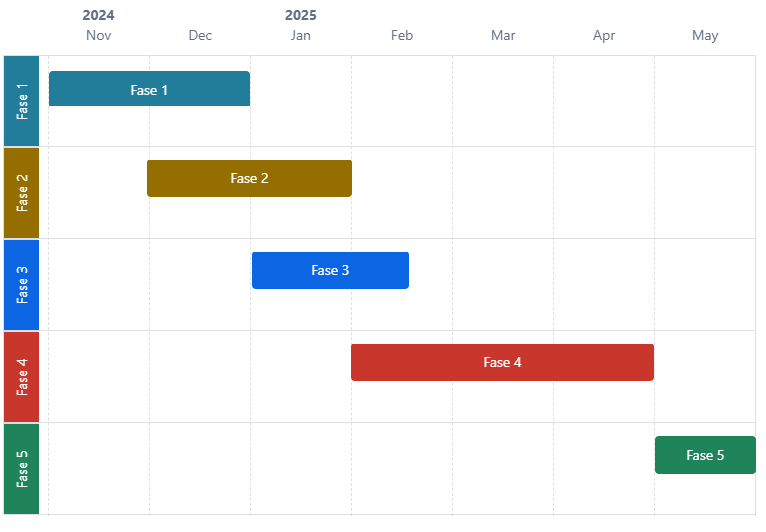
\includegraphics[width=.5\textwidth]{../graphics/Chart-Tijd-Visualisatie.png}
    \caption{Tijdsplanning van het project}
    \label{fig:tijdsplanning}
\end{figure}


%---------- Verwachte resultaten ----------------------------------------------
\section{Verwacht resultaat, conclusie}%
\label{sec:verwachte_resultaten}

De meerwaarde van deze bachelorproef voor de doelgroep, de Aquarius Zwemclub Lebbeke, is duidelijk: de implementatie van een robuuste cloudopslagoplossing zal niet alleen de werkprocessen voor de lesgevers verbeteren, maar ook de algehele efficiëntie van de club vergroten. Door de administratieve processen te automatiseren en beter beheersbaar te maken, wordt er tijdswinst geboekt, wat meer ruimte biedt voor de daadwerkelijke activiteiten van de club. Bovendien zal de verbetering van de toegang en beveiliging van documenten bijdragen aan een professionelere werking van de zwemclub.

De verwachte conclusie van deze bachelorproef is dan ook dat het gekozen cloudopslagsysteem zowel technisch haalbaar als praktisch effectief zal zijn voor de behoeften van de zwemclub. Mocht de gekozen oplossing echter niet voldoen aan de verwachtingen, dan zal het onderzoek zich richten op het identificeren van de tekortkomingen en de redenen waarom deze oplossing niet geschikt bleek. In dat geval zal er verder onderzocht worden welke alternatieven nog beter aansluiten bij de eisen van AZL.